%
% ---------------------------------------------------------------
% Copyright (C) 2012-2018 Gang Li
% ---------------------------------------------------------------
%
% This work is the default powerdot-tuliplab style test file and may be
% distributed and/or modified under the conditions of the LaTeX Project Public
% License, either version 1.3 of this license or (at your option) any later
% version. The latest version of this license is in
% http://www.latex-project.org/lppl.txt and version 1.3 or later is part of all
% distributions of LaTeX version 2003/12/01 or later.
%
% This work has the LPPL maintenance status "maintained".
%
% This Current Maintainer of this work is Gang Li.
%
%

\documentclass[
 size=14pt,
 paper=smartboard,  %a4paper, smartboard, screen
 mode=present, 		%present, handout, print
 display=slides, 	% slidesnotes, notes, slides
 style=tuliplab,  	% TULIP Lab style
 pauseslide,
 fleqn,leqno]{powerdot}


\usepackage{cancel}
\usepackage{caption}
\usepackage{stackengine}
\usepackage{smartdiagram}
\usepackage{attrib}
\usepackage{amssymb}
\usepackage{amsmath} 
\usepackage{amsthm} 
\usepackage{mathtools}
\usepackage{rotating}
\usepackage{graphicx}
\usepackage{boxedminipage}
\usepackage{rotate}
\usepackage{calc}
\usepackage[absolute]{textpos}
\usepackage{psfrag,overpic}
\usepackage{fouriernc}
\usepackage{pstricks,pst-3d,pst-grad,pstricks-add,pst-text,pst-node,pst-tree}
\usepackage{moreverb,epsfig,subfigure}
\usepackage{color}
\usepackage{booktabs}
\usepackage{etex}
\usepackage{breqn}
\usepackage{multirow}
\usepackage{natbib}
\usepackage{bibentry}
\usepackage{gitinfo2}
\usepackage{siunitx}
\usepackage{nicefrac}
%\usepackage{geometry}
%\geometry{verbose,letterpaper}
\usepackage{media9}
\usepackage{animate}
%\usepackage{movie15}
\usepackage{auto-pst-pdf}

\usepackage{breakurl}
\usepackage{fontawesome}
\usepackage{xcolor}
\usepackage{multicol}



\usepackage{verbatim}
\usepackage[utf8]{inputenc}
\usepackage{dtk-logos}
\usepackage{tikz}
\usepackage{adigraph}
%\usepackage{tkz-graph}
\usepackage{hyperref}
%\usepackage{ulem}
\usepackage{pgfplots}
\usepackage{verbatim}
\usepackage{fontawesome}


\usepackage{todonotes}
% \usepackage{pst-rel-points}
\usepackage{animate}
\usepackage{fontawesome}

\usepackage{listings}
\lstset{frameround=fttt,
frame=trBL,
stringstyle=\ttfamily,
backgroundcolor=\color{yellow!20},
basicstyle=\footnotesize\ttfamily}
\lstnewenvironment{code}{
\lstset{frame=single,escapeinside=`',
backgroundcolor=\color{yellow!20},
basicstyle=\footnotesize\ttfamily}
}{}


\usepackage{hyperref}
\hypersetup{ % TODO: PDF meta Data
  pdftitle={Presentation Title},
  pdfauthor={Gang Li},
  pdfpagemode={FullScreen},
  pdfborder={0 0 0}
}


% \usepackage{auto-pst-pdf}
% package to show source code

\definecolor{LightGray}{rgb}{0.9,0.9,0.9}
\newlength{\pixel}\setlength\pixel{0.000714285714\slidewidth}
\setlength{\TPHorizModule}{\slidewidth}
\setlength{\TPVertModule}{\slideheight}
\newcommand\highlight[1]{\fbox{#1}}
\newcommand\icite[1]{{\footnotesize [#1]}}

\newcommand\twotonebox[2]{\fcolorbox{pdcolor2}{pdcolor2}
{#1\vphantom{#2}}\fcolorbox{pdcolor2}{white}{#2\vphantom{#1}}}
\newcommand\twotoneboxo[2]{\fcolorbox{pdcolor2}{pdcolor2}
{#1}\fcolorbox{pdcolor2}{white}{#2}}
\newcommand\vpspace[1]{\vphantom{\vspace{#1}}}
\newcommand\hpspace[1]{\hphantom{\hspace{#1}}}
\newcommand\COMMENT[1]{}

\newcommand\placepos[3]{\hbox to\z@{\kern#1
        \raisebox{-#2}[\z@][\z@]{#3}\hss}\ignorespaces}
\renewcommand{\baselinestretch}{1.2}


\newcommand{\draftnote}[3]{
	\todo[author=#2,color=#1!30,size=\footnotesize]{\textsf{#3}}	}
% TODO: add yourself here:
%
\newcommand{\gangli}[1]{\draftnote{blue}{GLi:}{#1}}
\newcommand{\shaoni}[1]{\draftnote{green}{sn:}{#1}}
\newcommand{\gliMarker}
	{\todo[author=GLi,size=\tiny,inline,color=blue!40]
	{Gang Li has worked up to here.}}
\newcommand{\snMarker}
	{\todo[author=Sn,size=\tiny,inline,color=green!40]
	{Shaoni has worked up to here.}}

%%%%%%%%%%%%%%%%%%%%%%%%%%%%%%%%%%%%%%%%%%%%%%%%%%%%%%%%%%%%%%%%%%%%%%%%
% title
% TODO: Customize to your Own Title, Name, Address
%
\title{Twitter US Airline Sentiment}
\author{
  \\Shukai Wang
  \\Xi'an Shiyou University
}
\date{\today}

% Customize the setting of slides
\pdsetup{
% TODO: Customize the left footer, and right footer
rf=\href{http://www.tulip.org.au}{
Last Changed by: \textsc{\gitCommitterName}\ (\gitAuthorDate)
%Last Changed by: \textsc{\gitCommitterName}\ \gitVtagn-\gitAbbrevHash\ (\gitAuthorDate)
},
cf={Twitter US Airline Sentiment},
}


\begin{document}

\maketitle

%\begin{slide}{Overview}
%\tableofcontents[content=sections]
%\end{slide}


%%==========================================================================================
%%
\begin{slide}[toc=,bm=]{Table of content}
\tableofcontents[content=currentsection,type=1]
\end{slide}
%%
%%==========================================================================================


\section{Problem}


%%==========================================================================================
%%
\begin{slide}{Description}
  \begin{center}

    \twotonebox{\rotatebox{90}{Description}}{\parbox{.86\textwidth}
    {
      Sentiment analysis work on the issues of each major US airline. 
      Twitter counted the tweets related to airlines since February 2015,
       and analyzed whether the sentiments contained in these tweets were positive, neutral or negative.
      \begin{itemize}
        \item 
          Analyze how travelers in February 2015 expressed their feelings on Twitter.
      \end{itemize}
    }
    }

    \end{center}
    \bigskip
    \begin{center}
    \end{center}
    \bigskip
\end{slide}

%%==========================================================================================

\section{Data}


%%==========================================================================================
%%
\begin{slide}[toc=,bm=]{Basic Information of Data}
  
  \begin{table}[htbp]
  
    \caption{Train}
  
    \begin{tabular}{p{100pt} p{200pt}}\toprule
      Attribute & Explanation \\
         \midrule
         airline_sentiment
         & About the attitude of airlines. \\
         text
         & The text content of the tweet. \\
         airline
         & The name of the airline.  \\
         retweet_count
         & The number of reposts of the tweet.  \\
         tweet_created
         & The time the tweet was generated.  \\
        \bottomrule
    \end{tabular}
  \end{table}
  It also includes attributes such as tweet_id, 
  airline_sentiment_confidence, negativereason, 
  negativereason_confidence, airline_sentiment_gold, name, 
  negativereason_gold, tweet_coord, tweet_location, user_timezone, etc.

  \bigskip

\end{slide}

%%==========================================================================================

\section{Date Analysis}

\begin{slide}{Sentiment}
  \begin{itemize}
    \item Positive, negative and neutral emotions accounted for the number and proportion of the total number of people respectively. 
    Among them, the number of negative attitudes is the largest and the number of positive attitudes is the least.
  \end{itemize}
  \begin{figure}[htbp]
    \centering
    \begin{minipage}[t]{0.48\textwidth}
      \centering
      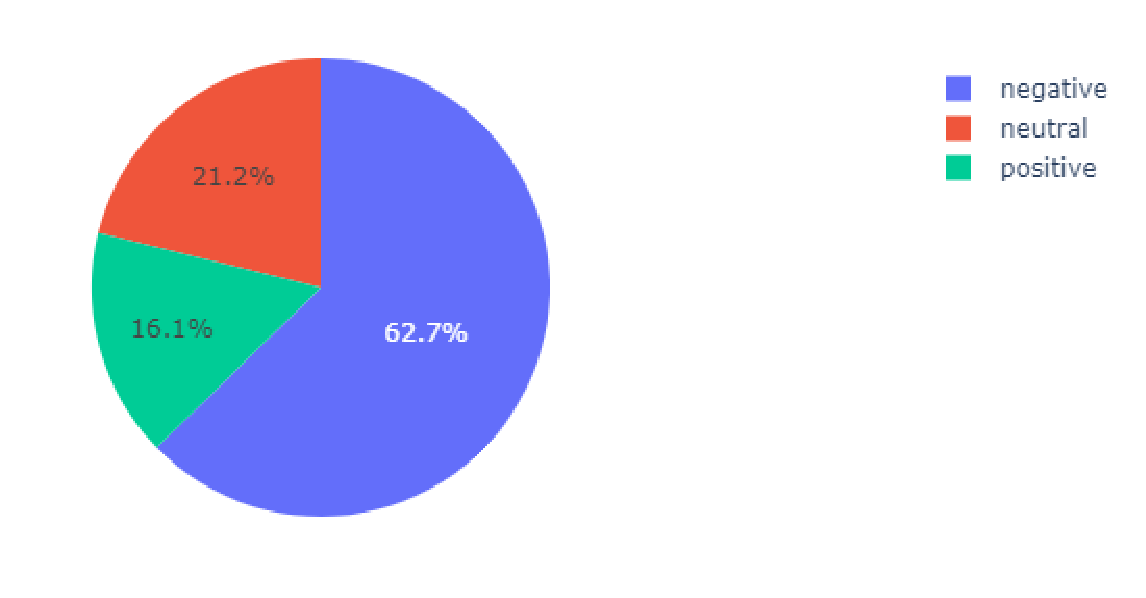
\includegraphics[width=0.9\textwidth]{figures//sentimentmap.eps}\\
      \vspace{-1.4em}
      \caption{Sentiment Map}
    \end{minipage}
    \begin{minipage}[t]{0.48\textwidth}
      \centering
      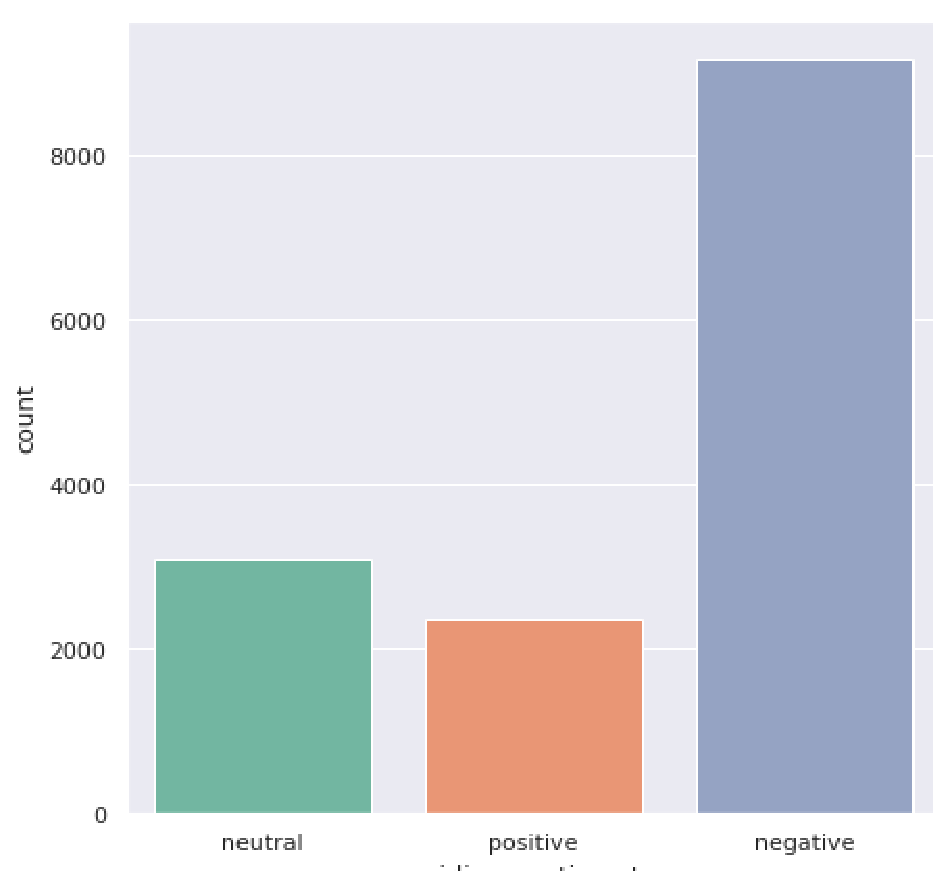
\includegraphics[width=0.9\textwidth]{figures//sentimentdist.eps}\\
      \vspace{-1.4em}
      \caption{Sentiment Dist}
    \end{minipage}
  \end{figure}
\end{slide}
%%
%%==========================================================================================


%%==========================================================================================
%%
\begin{slide}[toc=,bm=]{Airline}
  \begin{itemize}
    \item The percentage of each airline in all airlines.
  \end{itemize}
  
  \begin{figure}[htbp]
    \centering
    \begin{minipage}[t]{0.48\textwidth}
      \centering
      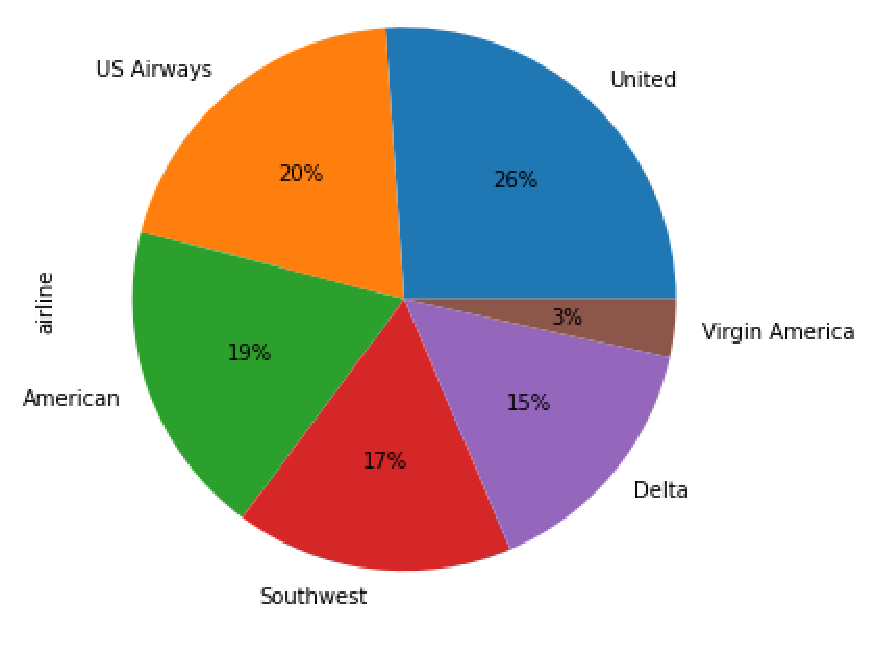
\includegraphics[width=0.9\textwidth]{figures//airlinemap.eps}\\
      \vspace{-1.4em}
      \caption{Airline Map}
    \end{minipage}
    \begin{minipage}[t]{0.48\textwidth}
      \centering
      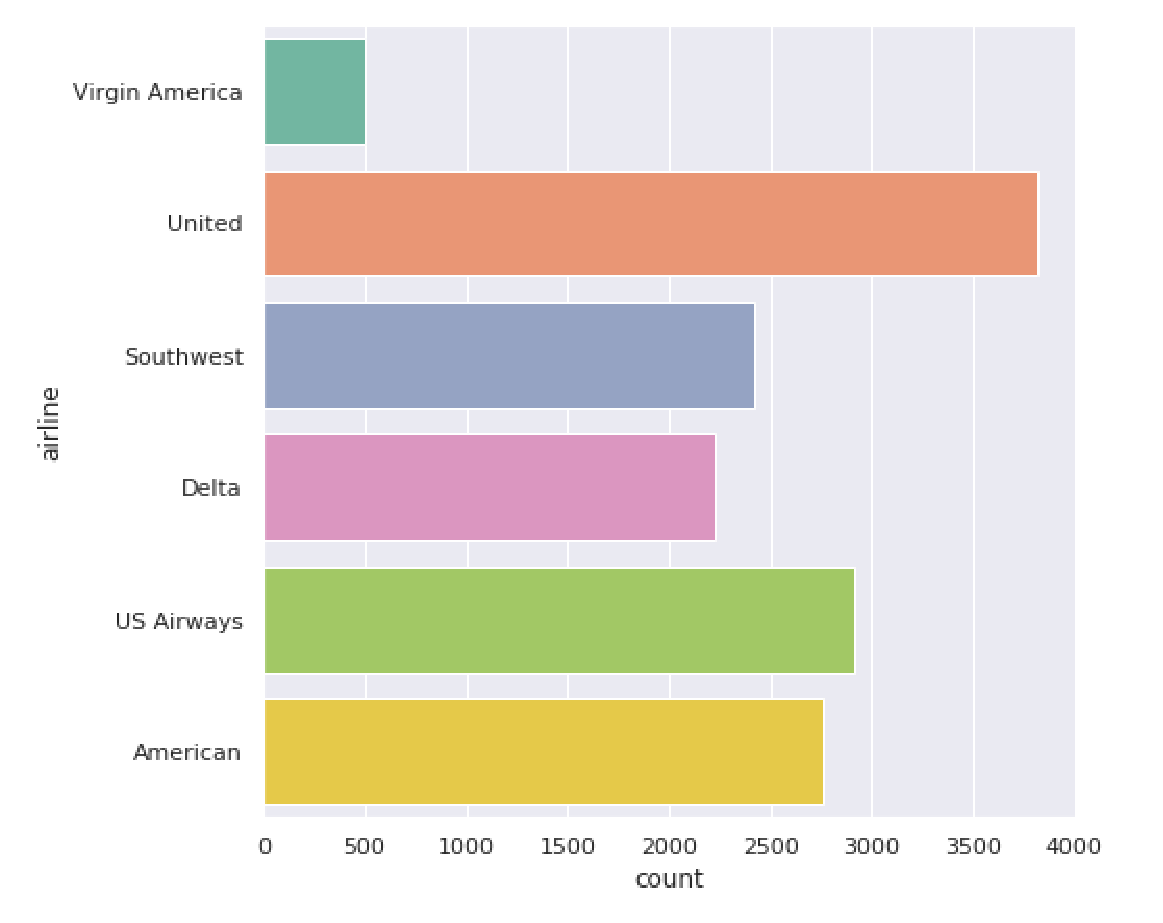
\includegraphics[width=0.9\textwidth]{figures//airlinedist.eps}\\
      \vspace{-1.4em}
      \caption{Airline Dist}
    \end{minipage}
  \end{figure}
%   \begin{figure}[htbp]
%     \centering
%     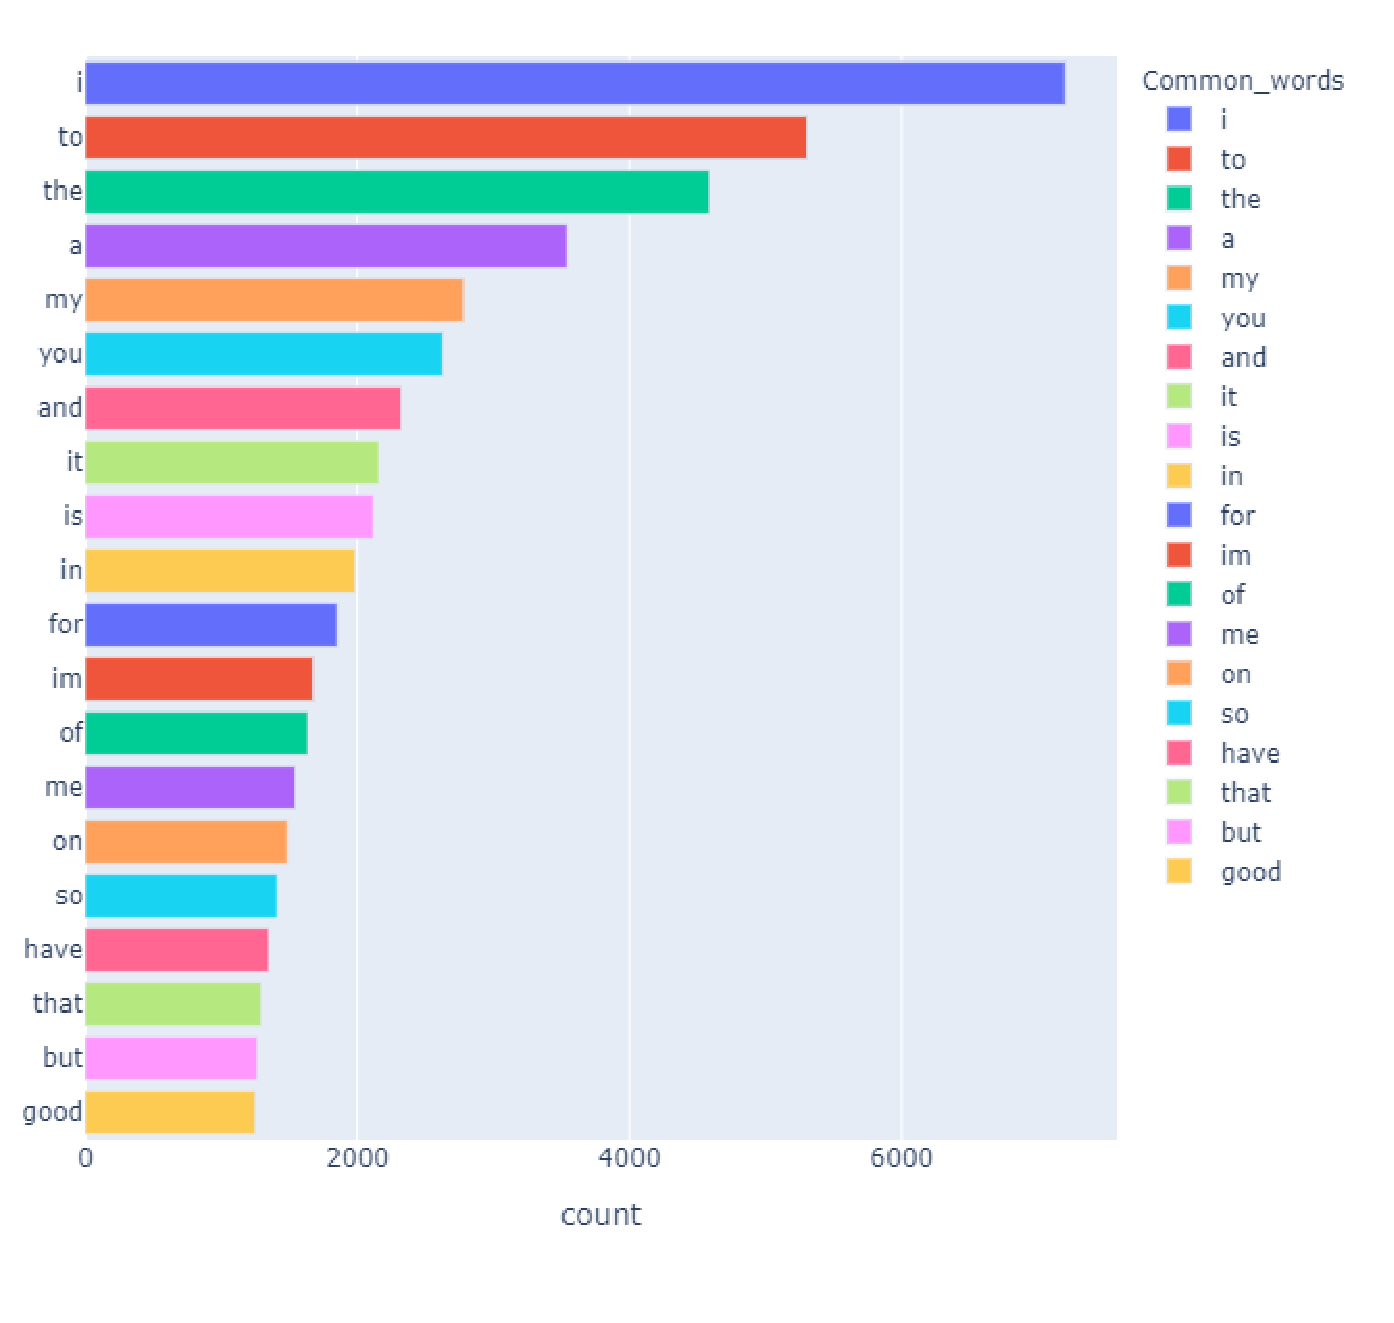
\includegraphics[width=0.5\textwidth]{figures//st_count_test.eps}
%     \caption{Select_text Count}
%   \end{figure}
\end{slide}
%%
%%==========================================================================================

\begin{slide}[toc=,bm=]{Airline Attitude}
  \begin{itemize}
    \item Distribution of attitudes of different airlines.
  \end{itemize}
  \begin{figure}[htbp]
    \centering
      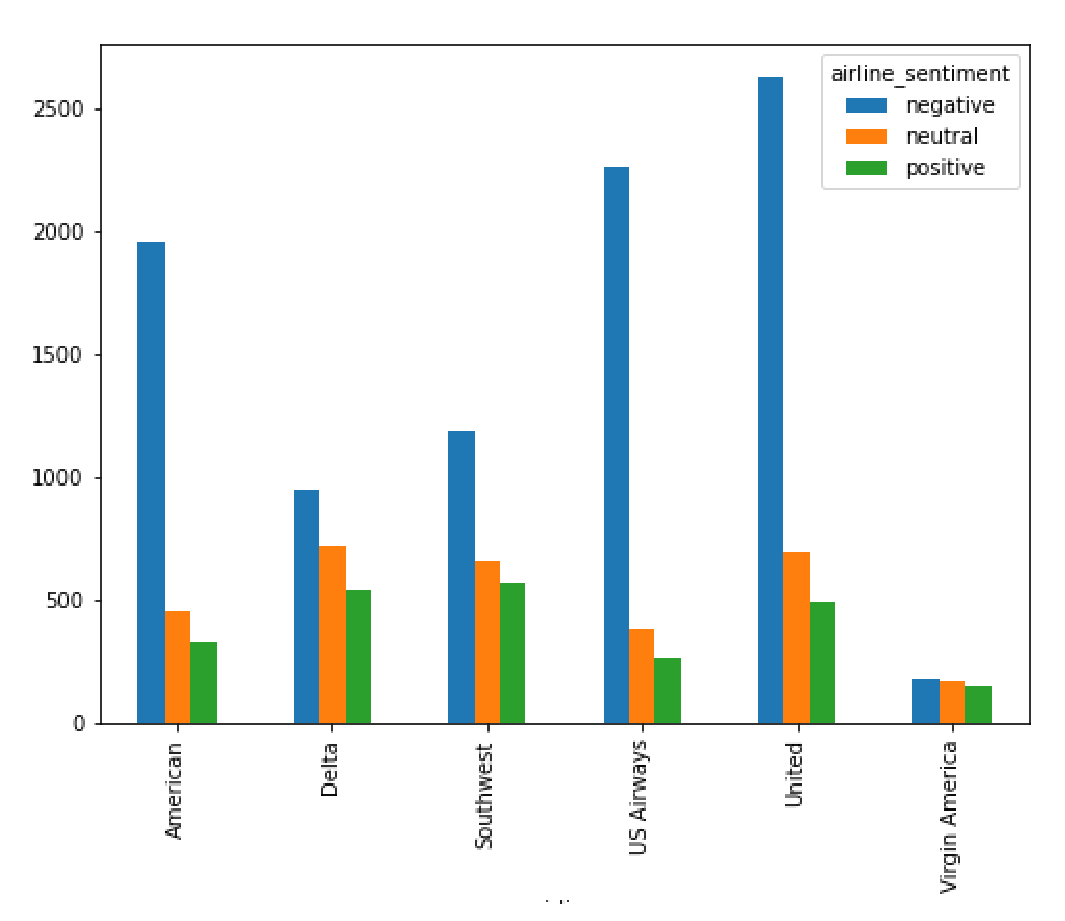
\includegraphics[width=0.5\textwidth]{figures//airlineattitude.eps}
      \caption{Airline Attitude}
 \end{figure}
\end{slide}


\begin{slide}{Airline Attitude}
  \begin{itemize}
    \item The individual attitude distribution of each airline.
  \end{itemize}
  \begin{figure}[htbp]
    \centering
    \begin{minipage}[t]{0.48\textwidth}
      \centering
      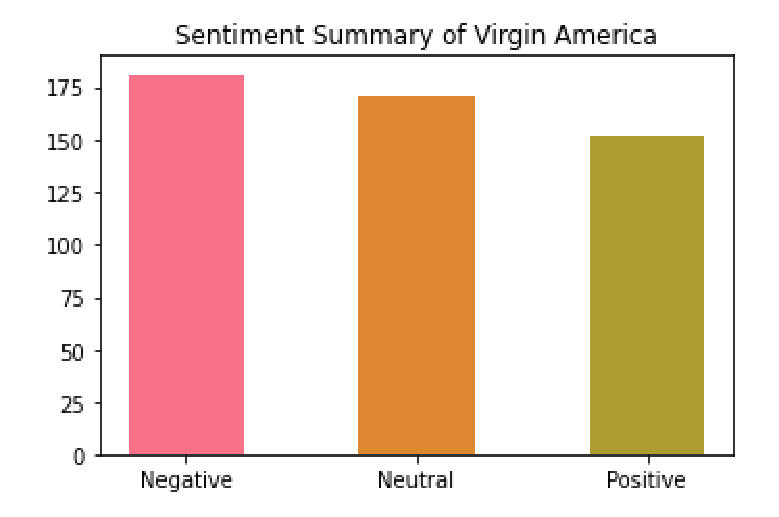
\includegraphics[width=0.9\textwidth]{figures//virgin.eps}\\
      \vspace{-1.4em}
      \caption{Virgin America}
    \end{minipage}
    \begin{minipage}[t]{0.48\textwidth}
      \centering
      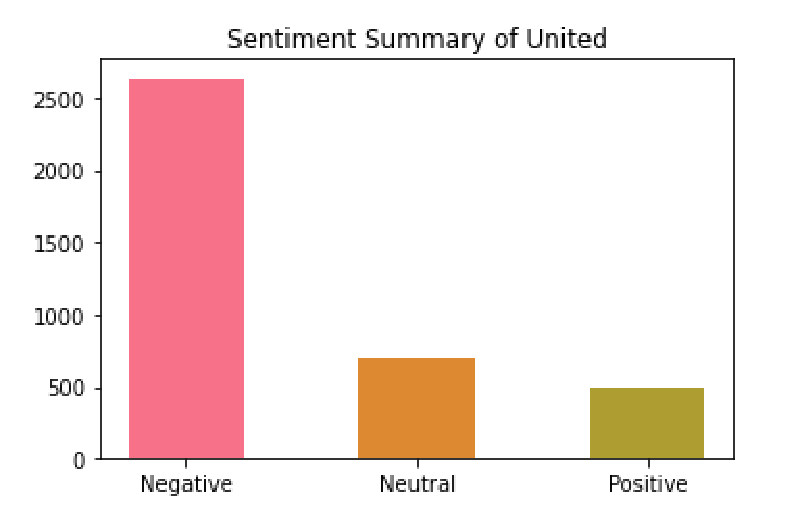
\includegraphics[width=0.9\textwidth]{figures//united.eps}\\
      \vspace{-1.4em}
      \caption{United}
    \end{minipage}
  \end{figure}
\end{slide}

\begin{slide}{Airline Attitude}
  % \begin{itemize}
  %   \item The individual attitude distribution of each airline.
  % \end{itemize}
  \begin{figure}[htbp]
    \centering
    \begin{minipage}[t]{0.48\textwidth}
      \centering
      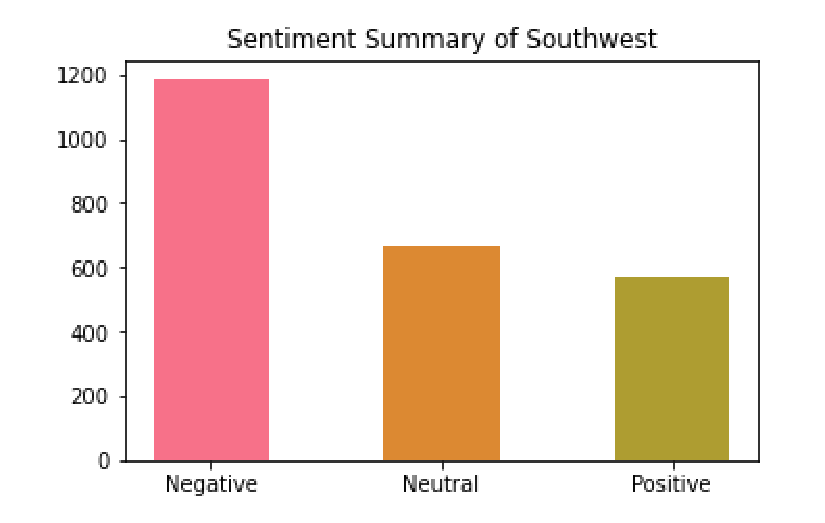
\includegraphics[width=0.9\textwidth]{figures//southwest.eps}\\
      \vspace{-1.4em}
      \caption{Southwest}
    \end{minipage}
    \begin{minipage}[t]{0.48\textwidth}
      \centering
      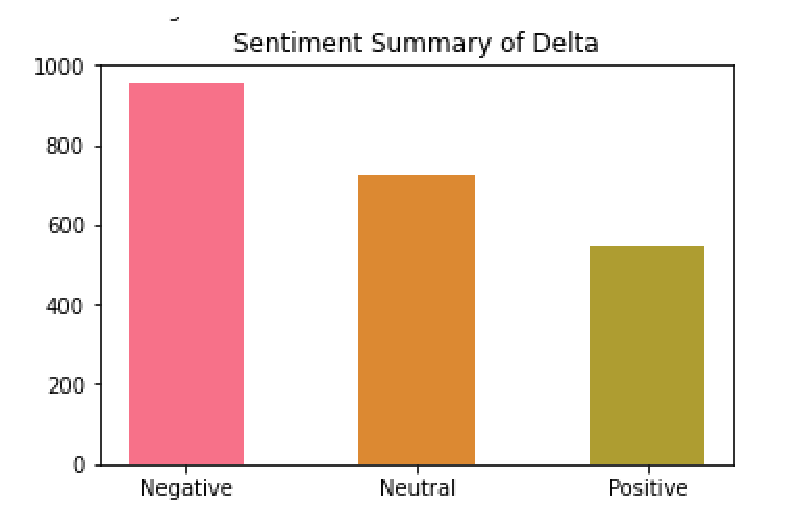
\includegraphics[width=0.9\textwidth]{figures//delta.eps}\\
      \vspace{-1.4em}
      \caption{Delta}
    \end{minipage}
  \end{figure}
\end{slide}

\begin{slide}{Airline Attitude}
  % \begin{itemize}
  %   \item The individual attitude distribution of each airline.
  % \end{itemize}
  \begin{figure}[htbp]
    \centering
    \begin{minipage}[t]{0.48\textwidth}
      \centering
      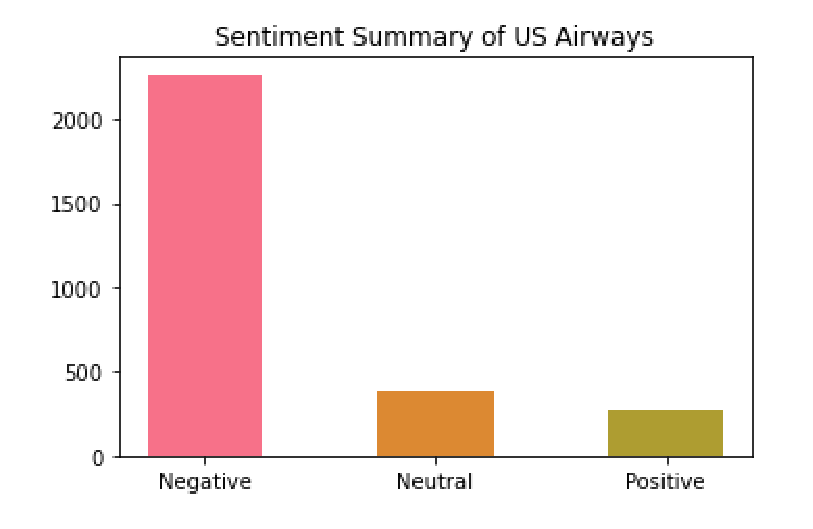
\includegraphics[width=0.9\textwidth]{figures//us.eps}\\
      \vspace{-1.4em}
      \caption{US Airways}
    \end{minipage}
    \begin{minipage}[t]{0.48\textwidth}
      \centering
      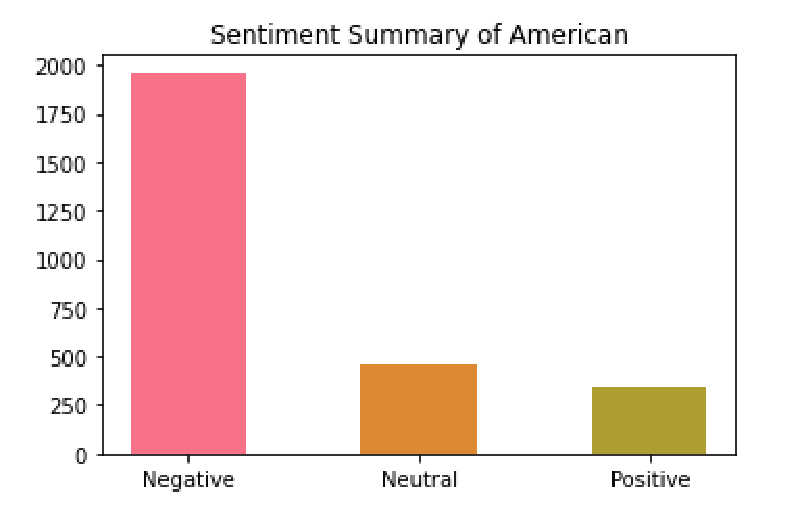
\includegraphics[width=0.9\textwidth]{figures//american.eps}\\
      \vspace{-1.4em}
      \caption{American}
    \end{minipage}
  \end{figure}
\end{slide}


\begin{slide}{negative Word Cloud}
  \begin{itemize}
    \item Words with negative emotions involve flight, canceled, hour, etc.
  \end{itemize}
  \begin{figure}[htbp]
    \centering
    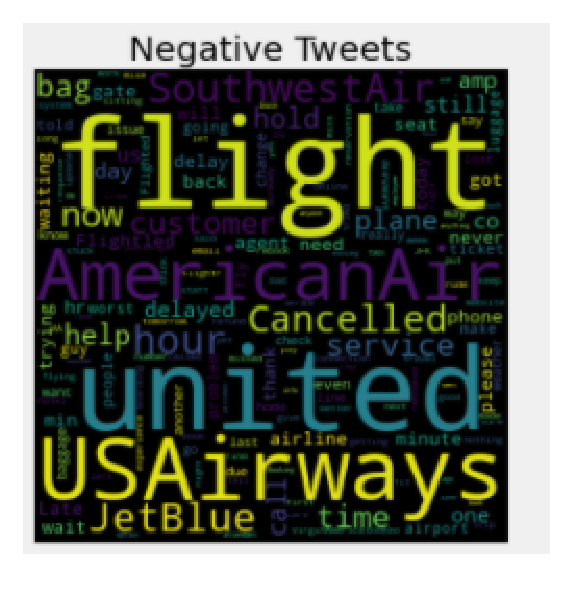
\includegraphics[width=0.4\textwidth]{figures//negativetweet.eps}
    \caption{Negative Words}
  \end{figure}
\end{slide}

\begin{slide}{Positive Word Cloud}
  \begin{itemize}
    \item Words with negative emotions include thanks, great, etc.
  \end{itemize}
  \begin{figure}[htbp]
    \centering
    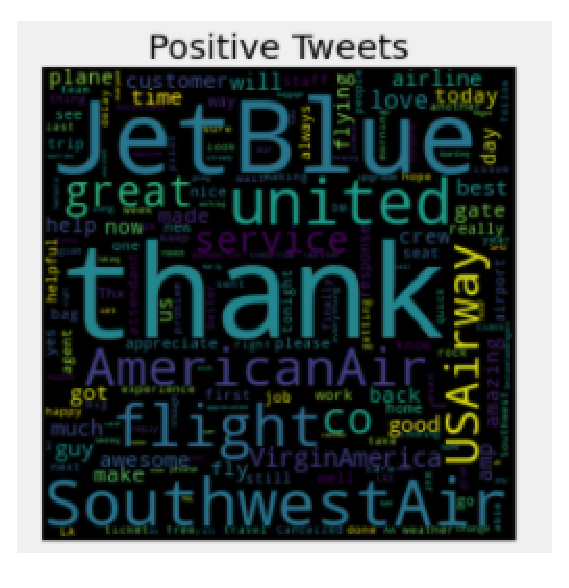
\includegraphics[width=0.4\textwidth]{figures//positiontweet.eps}
    \caption{Positive Words}
  \end{figure}
\end{slide}

\begin{slide}{Neutral Word Cloud}

  \begin{figure}[htbp]
    \centering
    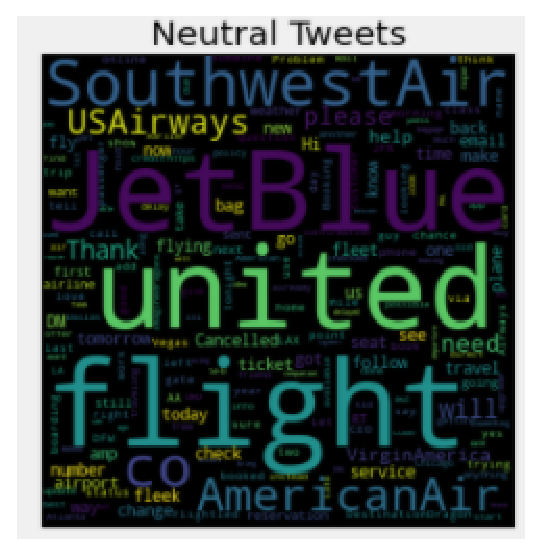
\includegraphics[width=0.4\textwidth]{figures//neutraltweet.eps}
    \caption{Neutral Words}
  \end{figure}
\end{slide}

\begin{slide}{Negative Reason}
  \begin{itemize}
    \item Perform statistical tactics on the causes of negative attitudes.
  \end{itemize}
  \begin{figure}[htbp]
    \centering
    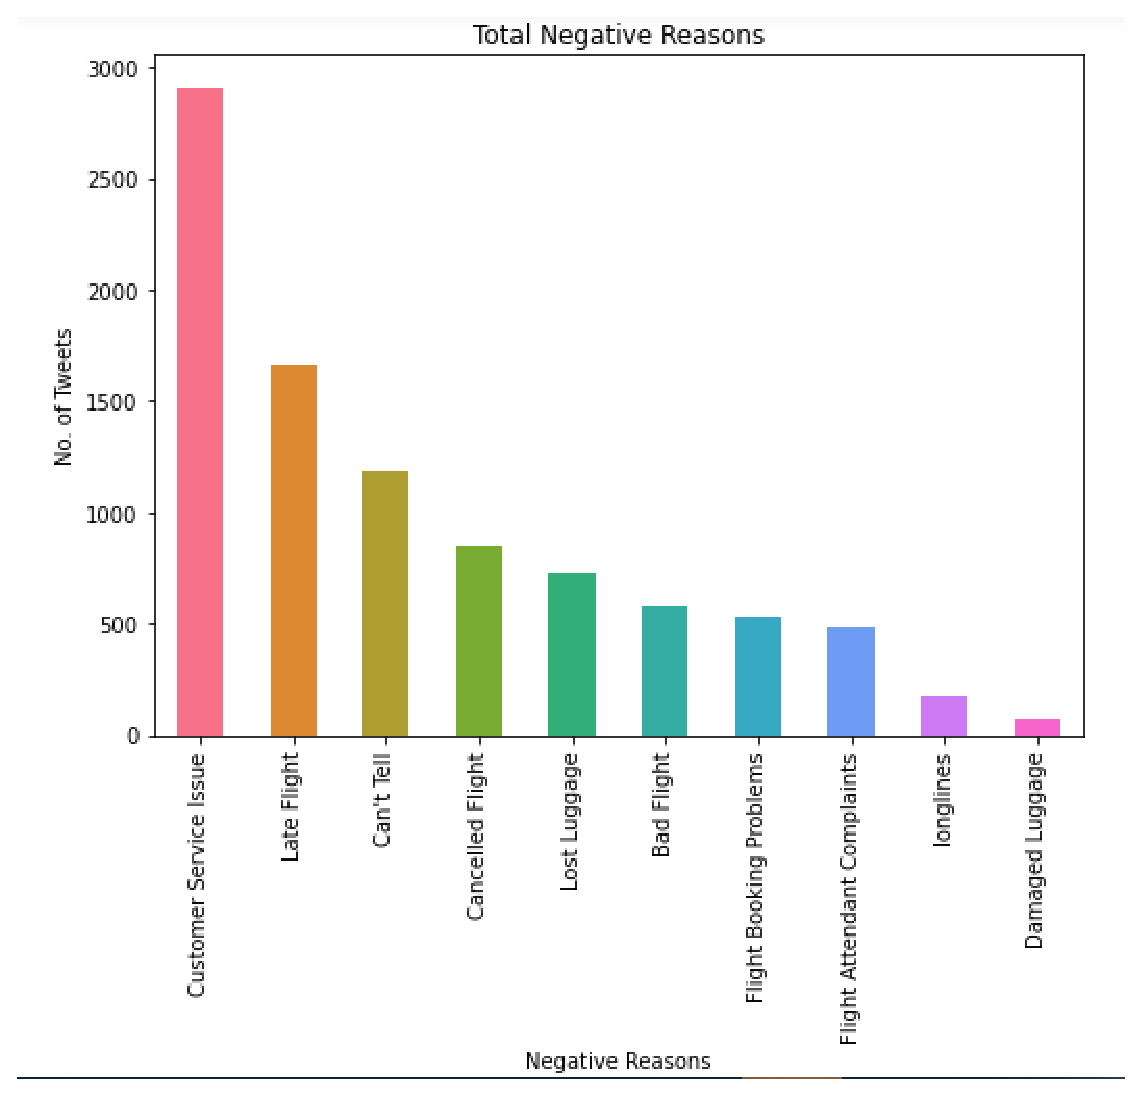
\includegraphics[width=0.5\textwidth]{figures//negativereason.eps}
    \caption{Total Negative Reasons}
  \end{figure}
\end{slide}



%%==========================================================================================
%%

% \begin{slide}[toc=,bm=]{Propaganda}
%   \begin{itemize}
%     \item Later stage propaganda has a great influence on the existing.
%   \end{itemize}
%   \begin{figure}[htbp]
%     \centering
%     \begin{minipage}[t]{0.48\textwidth}
%       \centering
%       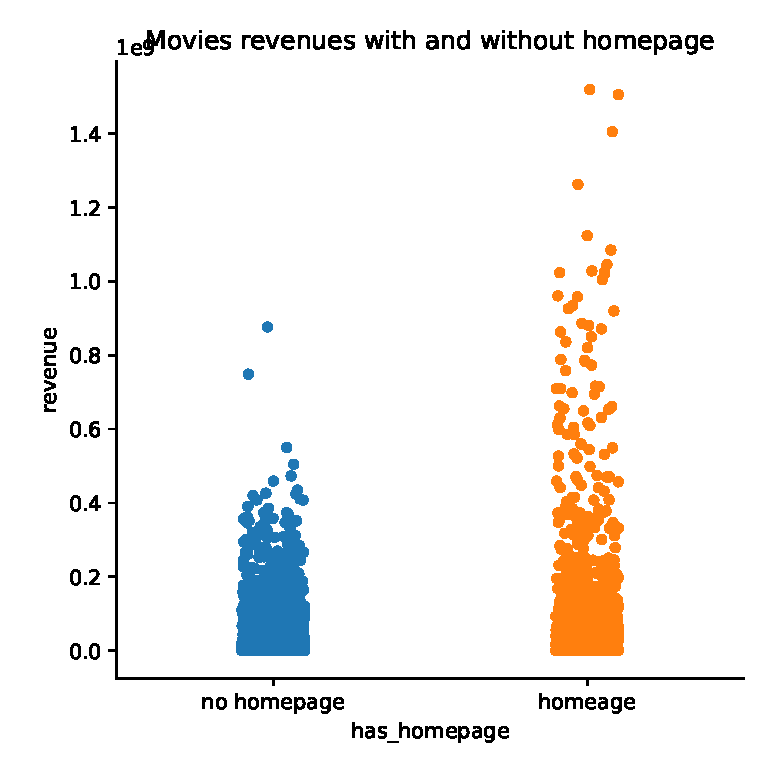
\includegraphics[width=0.4\textwidth]{figures/has_homepage.eps}
%       \vspace{-1.4em}
%       \caption{Homepage}
%     \end{minipage}
%     \begin{minipage}[t]{0.48\textwidth}
%       \centering
%       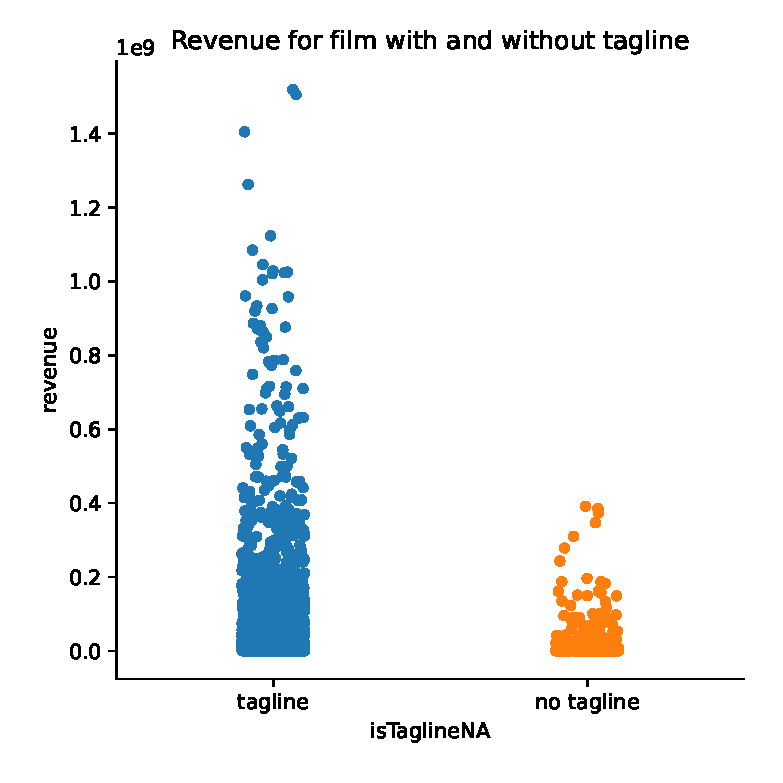
\includegraphics[width=0.4\textwidth]{figures/isTanglineNA.eps}
%       \vspace{-1.4em}
%       \caption{Tagline}
%     \end{minipage}
%     \begin{minipage}[t]{0.48\textwidth}
%       \centering
%       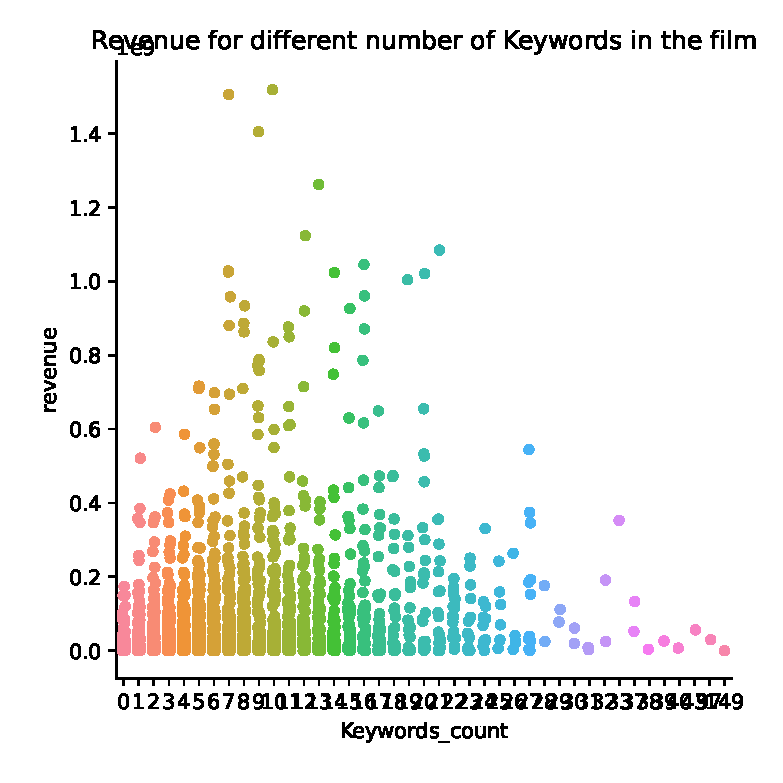
\includegraphics[width=0.5\textwidth]{figures/keywords.eps}
%       \vspace{-1.4em}
%       \caption{keywords}
%     \end{minipage}
%     \begin{minipage}[t]{0.48\textwidth}
%       \centering
%       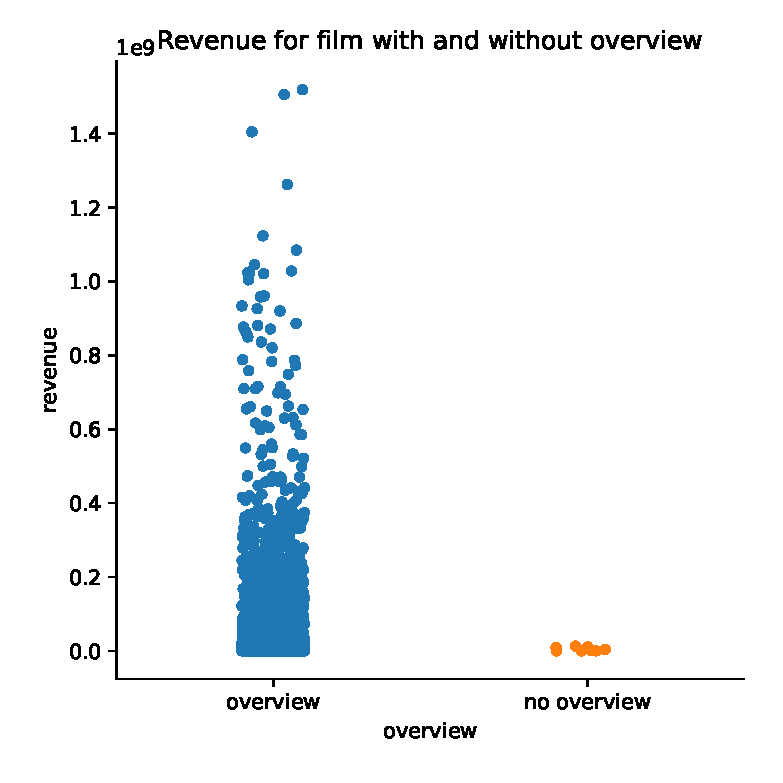
\includegraphics[width=0.5\textwidth]{figures/overview.eps}
%       \vspace{-1.4em}
%       \caption{Overview}
%     \end{minipage}
%   \end{figure}
% \end{slide}


%%==========================================================================================
%%
% \begin{slide}[toc=,bm=]{Realte Date}
% %  \begin{itemize}
% %    \item The income of the film is directly proportional to the budget.
% %  \end{itemize}
%   \begin{figure}[htbp]
%     \centering
%     \includegraphics[width=0.7\textwidth]{figures//release_date.eps}
%     \caption{Realte Date}
%   \end{figure}
% \end{slide}
% %%


\section{Data Processing}


\begin{slide}[toc=,bm=]{Data Processing}
  \begin{itemize}
    \item Processing data independent of results.
      \begin{itemize}
        \item For example:tweet_id,name,tweet_location,tweet_coord etc
      \end{itemize}
    \item  Normalization of training data and test data.
      \begin{itemize}
        \item For example:airline_sentiment,airline etc
      \end{itemize}
    \item Split train and test data.
  \end{itemize}
  % \begin{table}[htbp]
  %   \caption{Delete Data}
  %   \begin{tabular}{p{100pt} | p{200pt}}\toprule
  %    Name & Description  \\
  %        \midrule
  %        tweet_id
  %        & ID of movie in TMDB \\
  %        tweet_location
  %        & The original name of the movie\\
  %        poster_path
  %        & Movie poster link \\
  %        status
  %        &The state of the film \\
  %       \bottomrule
  %   \end{tabular}
  %  \end{table}
\end{slide}
%%


\section{Modeling}


%%
\begin{slide}[toc=,bm=]{Model}

\begin{itemize}
  \item Random Forest
    %  \begin{itemize}
    %    \item 2.4236034243650315
    %  \end{itemize}  
  \item Gradient Boosting
    %  \begin{itemize}
    %    \item 2.21274632296787
    %  \end{itemize}
  \item LSTM RNN
\end{itemize}

\begin{table}
\centering
\caption{Comparative Results}

\begin{tabular}{p{150pt} | p{200pt}}
\toprule
  Model & Accuracy\\
\hline
 Random Forest & 0.8135245901639344 \\
 Gradient Boosting & 0.8265027322404371  \\
 LSTM RNN & 0.8865852952003479  \\

\bottomrule

\end{tabular}
\end{table}

\end{slide}
%%
%%==========================================================================================



% %%
% \begin{slide}{Forecast}

% \begin{itemize}
% \item Random forest regression algorithm makes prediction.
% \end{itemize}

% \begin{table}
% \centering
% \caption{Forecast Results}

% \begin{tabular}{p{65pt} | p{110pt}}
% \toprule
%   id & revenue\\
% \hline
%   3001 & 193077.0567 \\
%   3002 & 528484.58  \\
%   3003 & 4562948.933  \\
%   3004 &  14433891.04 \\
%   3005 &  494782.0824  \\
%   3006 &  3010483.492  \\
% \bottomrule

% \end{tabular}
% \end{table}

% \end{slide}


% %%
% %%==========================================================================================


\section{Conclusion}

%%==========================================================================================
%%
\begin{slide}[toc=,bm=]{Conclusion}
\begin{itemize}
\item On this issue, the new model is better than the traditional machine learning model.
\smallskip

\item
\smallskip
Pay attention to the adjustment of parameters when training the model.

\item
\smallskip
Other models can be used to further improve accuracy.
\end{itemize}

\end{slide}
%%
%%==========================================================================================


%%==========================================================================================
% TODO: Contact Page
%\begin{wideslide}[toc=,bm=]{Contact Information}
%\centering
%\vspace{\stretch{1}}
%\twocolumn[
%lcolwidth=0.35\linewidth,
%rcolwidth=0.65\linewidth
%]
%{
% \centerline{\includegraphics[scale=.2]{tulip-logo.eps}}
%}
%{
%\vspace{\stretch{1}}
%Associate Professor Gang Li\\
%School of Information Technology\\
%Deakin University, Australia
%\begin{description}
% \item[\textcolor{orange}{\faEnvelope}] \href{mailto:gangli@tulip.org.au}
% {\textsc{\footnotesize{gangli@tulip.org.au}}}
%
% \item[\textcolor{orange}{\faHome}] \href{http://www.tulip.org.au}
% {\textsc{\footnotesize{Team for Universal Learning and Intelligent Processing}}}
%\end{description}
%}
%\vspace{\stretch{1}}
%\end{wideslide}
%
\end{document}

\endinput
